\documentclass[a4paper,12pt]{article}
\usepackage[utf8]{inputenc}
\usepackage{amssymb,amsmath,uniinput,graphicx,hyperref, multirow,units}
\usepackage[section]{placeins}
\usepackage[ngerman]{babel}
\usepackage[left=3cm,right=3cm,top=3cm,bottom=3cm]{geometry}
\renewcommand{\familydefault}{\sfdefault}
\setlength{\belowcaptionskip}{6pt}
\hypersetup{pdfinfo = {
	Title={Versuchsprotokoll zur Paulschen Teilchenfalle},
	Author={Knut Kiesel, Tobias Pook},
	Keywords={Teilchenfalle}
}}

\title{Laborpraktikum Teilchenphysik\\ Paulsche Teilchenfalle}
\author{Knut Kiesel\\Tobias Pook}
\date{\today}

\begin{document}
\maketitle
\vspace{5cm}
\tableofcontents
\thispagestyle{empty}
\newpage
\setcounter{page}{1}

\section{Ziel der Messung} % max 1 Seite
Ziel des Versuches ist die Speicherung von elektrisch geladenen Teilchen und die Bestimmung des Verhältnisses von Ladung zu Masse.
Um die Teilchen in einem räumlich begrenzten Feld zu halten, ist ein statisches elektrisches Feld nicht ausreichend, da man damit keine Potentialminima schaffen kann.
Eine Möglichkeit dennoch Teilchen zu fangen ist das Anlegen von phasenverschobenen Wechselspannungen und Gleichspannungen, wobei bei richtiger Einstellungen der Spannungen und Frequenzen die Teilchen stabil in der Falle bleiben.
Konkret wurden beim durchgeführten Experiment der meta-stabile Bereich eines rotierenden Sattelpotential genutzt um Teilchen zu speichern.
Für jede räumliche Komponente $i\in\{x,y,z\}$ lautet die Bewegungsgleichung
\begin{align}\label{mastergleichung}
	\frac{4}{mΩ^2} |\vec{F}_i| + \left( a_i -2q_i \cos\left( 2\xi_i \right) \right) i  + 2k_L \frac{dx}{d\xi_i} + \frac{d^2x}{d\xi_i^2} = B\cos\left( \frac{2ω_W}{Ω}ξ_i \right)
\end{align}
mit dem gleichstromabhängigen Koeffizienten $a_i = \frac{16KqU_{G,i}}{3Ω^2mr_0^2}$,
dem wechselstromabhängigen Koeffizienten  $q_i = -\frac{4kqU_i}{Ω^2mr_0^2}$,
dem Antribskoeffienzenten $B = \frac{2qU_W}{r_0mΩ^2}$,
dem Luftreibungskoeffizient $k_L = \frac{6πηR}{mΩ}$, der Winkelfrequenz der Dreiphasenspannung $Ω$,
der Winkelfrequenz der zusätzlich an einem Plattenpaar angelegten Wechselspannung $ω_W$
und der normalisierten Zeit $ξ = \frac{Ωt}{2}$.
$\vec{F}$ ist eine konstante äußere Kraft, zum Beispiel bei der z-Komponente die Gewichtskraft.
Die Grundschwingung der Lösung wird durch
$$β_i = \sqrt{a_i + \frac{q_i^2}{2}}$$
beschrieben.
Durch Anlegen geeigneter Frequenzen und Spannungen und das Beobachten der entstehenden Teilchenbewegungen kann mit unterschiedlichen Methoden das Verhältnis von Ladung zur Masse bestimmt werden.


\section{Aufbau und Durchführung}
Die z-Achse verläuft vertikal, die y-Achse ist die Blickrichtung, und die x-Achse liegt senkrecht zu den beiden übrigen.

Die Falle wird aus sechs Kupferringen und 12 Verbindungsstücken zu einem Würfel geklebt.
Nach dem Anlöten und Isolieren der Anschlusskabel wird die Falle mit schwarzem Lack angestrichen, um Steulicht in der Kammer zu verringern.
Die Falle wird mittig über der Öffnung für die Spritze an den Anschlusskabeln befestigt und die Plattform von unten an die Spannungsversorgung angeschlossen (siehe Bild \ref{fallenbild}), welche je nach Hebelstellung die Gleichspannungen oder die zusätzliche Wechselspannung zur Dreiphasenspannung hinzufügt.
Die Dreiphasenspannung, im folgenden auch Fokussierspannung genannt, wird aus drei Wechselpannungsquellen die mit einem konstanten Phasenunterschied von $120^\circ$ betrieben werden, geliefert.
Die Amplitude kann dabei für jedes Flächenpaar individuell eingestellt werden.

\begin{figure}[htb]
		\centering
		\includegraphics[width=0.3\textwidth]{falle.jpg}
		\caption{Versuchsaufbau der Paulschen Teilchenfalle}
		\label{fallenbild}
\end{figure}

Es gibt mehrere Möglichkeiten die Gleichspannung anzulegen:
Man kann sie auf den beiden gegenüber liegenden Seiten oder zwischen zwei gegenüberliegenden Seiten anbringen.
Die Verschaltung ist jedoch schon vorgefertigt und kann mit Schaltern hinzugeschaltet werden.
Die Verschaltung kann man Bild \ref{verschaltung} entnehmen.
\begin{figure}[htb]
		\centering
		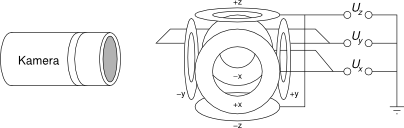
\includegraphics{Schaltbild_3Phasen.png}
		% hier fehlt noch die verschaltung der gleichspannung bzw der anderen spannungen. entweder packen wir hier noch die anderen bilder, oder wir bearbeiten das bild entsprechend.
		\caption{Verschaltung im Generator}
		\label{verschaltung}
\end{figure}

Aus Sicherheitsgründen wird die Falle durch eine durchsichtige Acrylhaube abgedeckt.
Die Haube wurde zusätzlich mit Ausnahme von zwei Stellen mit schwarzem Klebeband verkleidet.
Die zwei Öffnungen dienen der seitlichen Beobachtung der Falle und der Bestrahlung durch eine oben angebrachten Lampe.
Die geladen Teilchen sind Aluminiumpulverstücke, die mittels einer Spritze durch eine Öffnung unterhalb der Falle eingebracht werden.
Durch das Reiben an der Spritzenöffnung werden die Aluminiumteile ionisiert.
Da zwischen Öffnung und dem stabilen Bereich der Teilchenfalle ein Abstand von ca. $\unit[2.5]{cm}$  besteht wurden die Teilchen durch anschnipsen der Spritze in die Falle geschleudert.



\section{Ergebnisse}
Mit einem Messschieber wird der Plattenabstand der Teilchenfalle auf $d = \unit[(3.05±0.02)]{cm}$ abgeschätzt.
\subsection{Bahnbeschreibung}
In den meisten Fällen beschreiben die eingefangenen Teilchen eine elliptische Teilchenbahn deren Radius und die Exzentrizität durch das Verhältnis der angelegten Potenziale in der Fokusierspannung erklärt werden können.
Viele Teilchen beschreiben zudem sehr kleine Bahnen und sind deshalb nur noch als Punkte wahrzunehmen.

Manchmal bilden sich auch Lissajou Figuren. Lissajous Figuren entstehen bei der Überlagerung harmonischer Schwingungen, wenn das Verhältnis der Frequenzen rational ist.
In diesem Fall bildet die Teilchenbahn eine geschlossene Figur.
Die möglichen Formen der Figuren sind sehr vielfältig und hängen vom Frequenzverhältnis und dem Phasenunterschied der Schwingungen ab.
Ein Beispiel ist in Bild \ref{Lissjous} zu sehen.

\begin{figure}[htb]
		\centering
		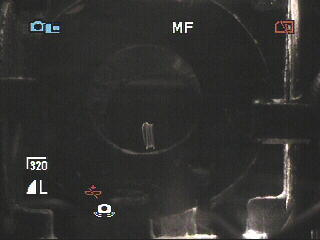
\includegraphics{lisa1.jpg}
		\caption{Beispiel für das auftreten einer Lissajous Figur}
		\label{Lissjous}
\end{figure}

Wenn man mehrere Teilchen in der Teilchenfalle gefangen hat, kann man manchmal pseudo Kristallstrukturen erkennen:
Die Teilchen stoßen sich gegenseitig ab und suchen energetisch günstige Zustände, ebenso wie in einem Kristall.
Maximal wurden vier Teilchen auf einmal eingefangen, die alle ähnliche Abstände zueinander hatten, leider sind das noch zu wenige, um eine definitive Aussage über die genaue Kristallstruktur zu machen.

\subsection{Kompensation der Gewichtskraft}
In Gleichung (\ref{mastergleichung}) wird der Einfluss der Luftreibung vernachlässigt und ein Näherungsansatz der Form $z(ξ_z) = Z(ξ_z)+d(ξ_z)$ durchgeführt.
Die z-Komponente wird nun durch
\begin{align*}
	Z(ξ) = Z_0\sin(β_zξ) - \frac{4|\vec{F}_z|}{mβ_zΩ^2}
\end{align*}
beschrieben.
Man sieht, dass die Schwingung um einen konstanten Term verschoben ist, der von $a_z$ und $q_z$ abhängt.
Diese Abhängigkeit besteht nicht mehr, wenn gilt:
\begin{align}
	\label{kraftgleichgew}
	|\vec{F}_{z}| = |\vec{F}_G + \vec{F}_{qE}| = mg + q\frac{U_G}{d} = 0
\end{align}

\begin{figure}[htb]
		\centering
		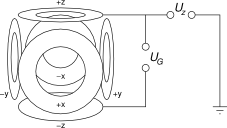
\includegraphics{Schaltbild_Z_Kompensation.png}
		\caption{Schaltbild Z-Kompensation}
		\label{schalt-z}
		% wollen wir die schlaltung oben beim versuchsaufbau erklären?
\end{figure}

Zu der Dreiphasenspannung wird nun ein zusätzlicher Potentialunterschied zwischen den beiden z-Komponenten angeschlossen (siehe Bild \ref{schalt-z}), der solange erhöht wird, bis die Gravitationskraft kompensiert wird.
Dies kann dadurch überprüft werden, dass sich der Mittelpunkt der Teilchenschwingung bei Änderung der Amplitude der z-Komponente der Dreiphasenspannung nicht mehr ändert.
Die Fokussierspannung wird bei $U_i = \unit[(1000±50)]{V}$ für alle Flächenpaare betrieben.

Weil die Gleichspannung stark schwankend ist, wird die effektive Spannung durch notieren der angezeigten Werte in einem Zeitraum von ungefähr $\unit[20]{s}$ und anschliessendem Mitteln bestimmt.
Da man die Teilchen oft wegen spontaner Spannugsschwankungen der Quelle verliert, kann der Bereich, in dem die Gravitationskraft kompensiert wird, nicht in feineren Spannungsabschnitten untersucht werden.
Da so nicht abzuschätzen ist wie exakt der Wert für die Kompensationsspannung $U_G$ getroffen wird,
wird als Fehler die mittlere Differenz zu den nächstliegenden $U_G$ gewählt, bei dem wieder Bewegungen des Schwingungsmittelpunkt bei Variation der Fokussierspannung $U_z$ zu beobachten sind.
Die Messung wurde für mehrere gleichzeitig gefangene Teilchen durchgeführt und die Spannung erhöht bis alle Teilchen den Stabilitätsbereich verlassen haben.
Das Vorzeichen der Ladung ergibt sich aus dem Anschluss an die Spannungsquelle und ist für alle beobachteten Teilchen negativ, was mit der Theorie übereinstimmt.

\begin{table}
	\centering
	\begin{tabular}{ l | c | l | l }
		$U_{G} [V]$ & $\sigma_{U_{G}}[V]$ & \multicolumn{2}{l}{Verhalten des Bahnmittelpunkts bei Änderung von $U_z$}  \\
		\hline
		45 & 5 & Bewegung &  Bewegung   \\
		92 & 8 & still  & Bewegung \\
		168 & 4 & Bewegung & Bewegung    \\
		228 & 3 & Bewegung & Bewegung \\
		273 & 5 & verloren & still \\
	\end{tabular}
\caption{Verhalten von beiden Teilchen bei unterschiedlichen Gleichspannungen zur Bestimmung der z-Kompensation}
\label{tab:z-komp-measure}
\end{table}

Aus Gleichung \ref{kraftgleichgew} lässt sich direkt eine Formel für die spezifische Ladung des untersuchten Teilchen herleiten:
\begin{align}\label{zspezm}
	\frac{q}{m} = -\frac{g \cdot  d}{U_{G}}
\end{align}
wobei $g = \unitfrac[9.81]{m}{s^2}$ die Erdbeschleunigung ist und als fehlerfrei angenommen wird.
Die errechneten Werte können Tabelle \ref{tab:z-komp-result} entnommen werden.


\begin{table}
	\centering
	\begin{tabular}{ l | c | c }
		Teilchen &$U_{G,komp} [V]$ & $\frac{q}{m}[\frac{mC}{kg}]$  \\
		\hline
		1 &  92 ± 8 &  0.33 ± 0.04  \\
		\hline
		2 & 273 ± 5 &  0.109 ± 0.009  \\
	\end{tabular}
\caption{Das Verhältnis von Ladung zu Masse von verschiedenen Teichen, bestimmt durch die Kompensation der Gewichtskraft}
\label{tab:z-komp-result}
\end{table}

\subsection{Resonanz}
In diesem Versuchsteil wurde zusätzlich zur Fokusierspannung  eine Wechselspannung zwischen dem Flächenpaar entlang der x-Achse angelegt.
Die Gleichspannung wird auf $0$ geregelt.

%%%%%% Warum brauchen wir die ganzen Gleichungen???
%Damit vereinfacht sich Gleichung (\ref{mastergleichung}) zu
%\begin{align}\label{resgleichung}
%	\left( a_i -2q_i \cos\left( 2\xi_i \right) \right) i  + 2k_L \frac{dx}{d\xi_i} + \frac{d^2x}{d\xi_i^2} = B\cos\left( \frac{2ω_W}{Ω}ξ_i \right).
%\end{align}
%Die Teilchenbahn wird also durch eine erzwungene Schwingung moduliert, die Lösung von \ref{resgleichung} ist gegben durch:
%\begin{align}\label{resgleichung}
%	X(\xi_x) = X_0( \beta_x,\omega_W ) \cdot B \cdot cos(2\frac{\omega_W}{\Omega}\xi_x - \Phi(\beta_x,\omega_W))
%	\\
%	 tan\Phi(\beta_x,\omega_W) = \frac{4 k_L \Omega \omega_W}{\beta_x^{2}\Omega_x^{2}}
%	 \\
%	  X_0 = \frac{1}{\sqrt{16\omega^{4}_W\Omega^{-4}+\beta^{4}_x+16\Omega^{-2}k_L\omega^{2}_W-8\Omega^{-2}\beta^{2}_x\omega^{2}_W}}
%\end{align}
Bei einer Frequenz von
\begin{align}\label{w_res}
	\omega^{res}_W = \frac{\Omega}{2}\sqrt{\beta^{2}_x-2k^{2}_L}
\end{align}
tritt eine resonante Verstärkung der Oszillation auf und die Teilchenbahn erreicht ihre maximale Auslenkung
\begin{align}\label{Amax}
	A_{max} = \frac{B}{2k_L\sqrt{\beta^{2}_x-k^{2}_L}}.
\end{align}
Durch Eliminieren von $k_L$ in Gleichung \ref{w_res} und \ref{Amax} erhält man
\begin{align}\label{res_luft}
	\frac{q}{m} = ±\sqrt{
		\frac{
			U_w^2r^6Ω^4 ± r^4Ω^2\sqrt{
				(U_wrΩ)^4 - 4(4KU_xA_{max}ω)^4
			} %sqrt
		}{
			128A_{max}^2(KU_x)^4
		} % frac
	}. % sqrt
\end{align}
Für die Lösung im Vakuum reicht es in Gleichung (\ref{w_res}) $k_L=0$ zu setzen, und man erhält
\begin{align}\label{res_vak}
	\frac{q}{m} = -\frac{\Omega r^{2}_0 \omega^{res}_W}{\sqrt{2} K U_x}.
\end{align}

Um die Resonanzfrequenz zu messen, wird die Wechselspannung variiert bis das Teilchen maximale Auslenkung zeigt.
In Luft wird zusätzlich die maximale Amplitude bestimmt, indem mit einer Digitalkamera Fotos der Teilchenbahn angefertigt werden.
Es wird vor Durchführung des Versuchs die Falle entfernt und eine Längenskala auf Höhe der Fallenmitte senkrecht zur Kamerablickrichtung platziert und ein Vergleichsbild aufgenommen.
Da sowohl die Kameraposition, Kameraeinstellungen als auch die Teilchenfalle nicht mehr bewegt werden,
kann aus diesen Bildern ein Zusammenhang zwischen Pixeln pro cm in der Beobachtungsebene bestimmt werden.



%%%Ergebnisse

\subsubsection{Messung in Luft}
Wenn man die Ladung zu Masse Verhältnisse in Luft mit Gleichung (\ref{res_luft}) ausrechnet, erhält man zwei Lösungen, von der man diejenige nimmt, die näher am genäherten Wert von Gleichung (\ref{res_vak}) liegt.
Der Fehler beider Lösungen ist fast immer in der gleichen Größenordnung wie der Wert.
Dies liegt daran, dass die Formel Differenzen von hohen Potenzen beinhaltet, was einen großen relativen Fehler ergibt.



\subsection{Stabilitätsdiagramm}
Wie Gleichung (\ref{mastergleichung}) zu entnehmen, ist die Grundschwingung der Teilchen gegeben durch $β$.
Wenn $β$ imaginär ist ($ \Leftrightarrow a + \frac12q^2 >0$), werden die Winkelfunktionen zu Expotentialfunktionen, was zum Austritt der Teilchen aus der Falle führt.
Dafür wird bei verschiedenen, konstanten $U_x = U_y = U_z$ die Spannung $U_G$ gesucht, bei der das Teilchen entkommt.
Weil das Teilchen nicht entkommen darf (es muss bei mehreren $U_i$ vermessen werden), ist die Abschätzung nur schwer zu bewerkstelligen, da die Gleichspannungsquelle stark schwankt und es somit leicht entkommen kann.
Für jedes Teilchen wird $U_g$ gegen $U_i^2$ aufgetragen und eine lineare Regression durchgeführt.
Die systematischen Fehler für das grobe Abschätzen der Gleichspannung resultieren sich in einer Verschiebung der Geraden nach unten, sodass die Steigung nicht stark beeinflusst wird.
Aus der Steigung kann man dann die Werte für $\frac{q}{m}$ bestimmen.
\begin{figure}[htb]
		\centering
		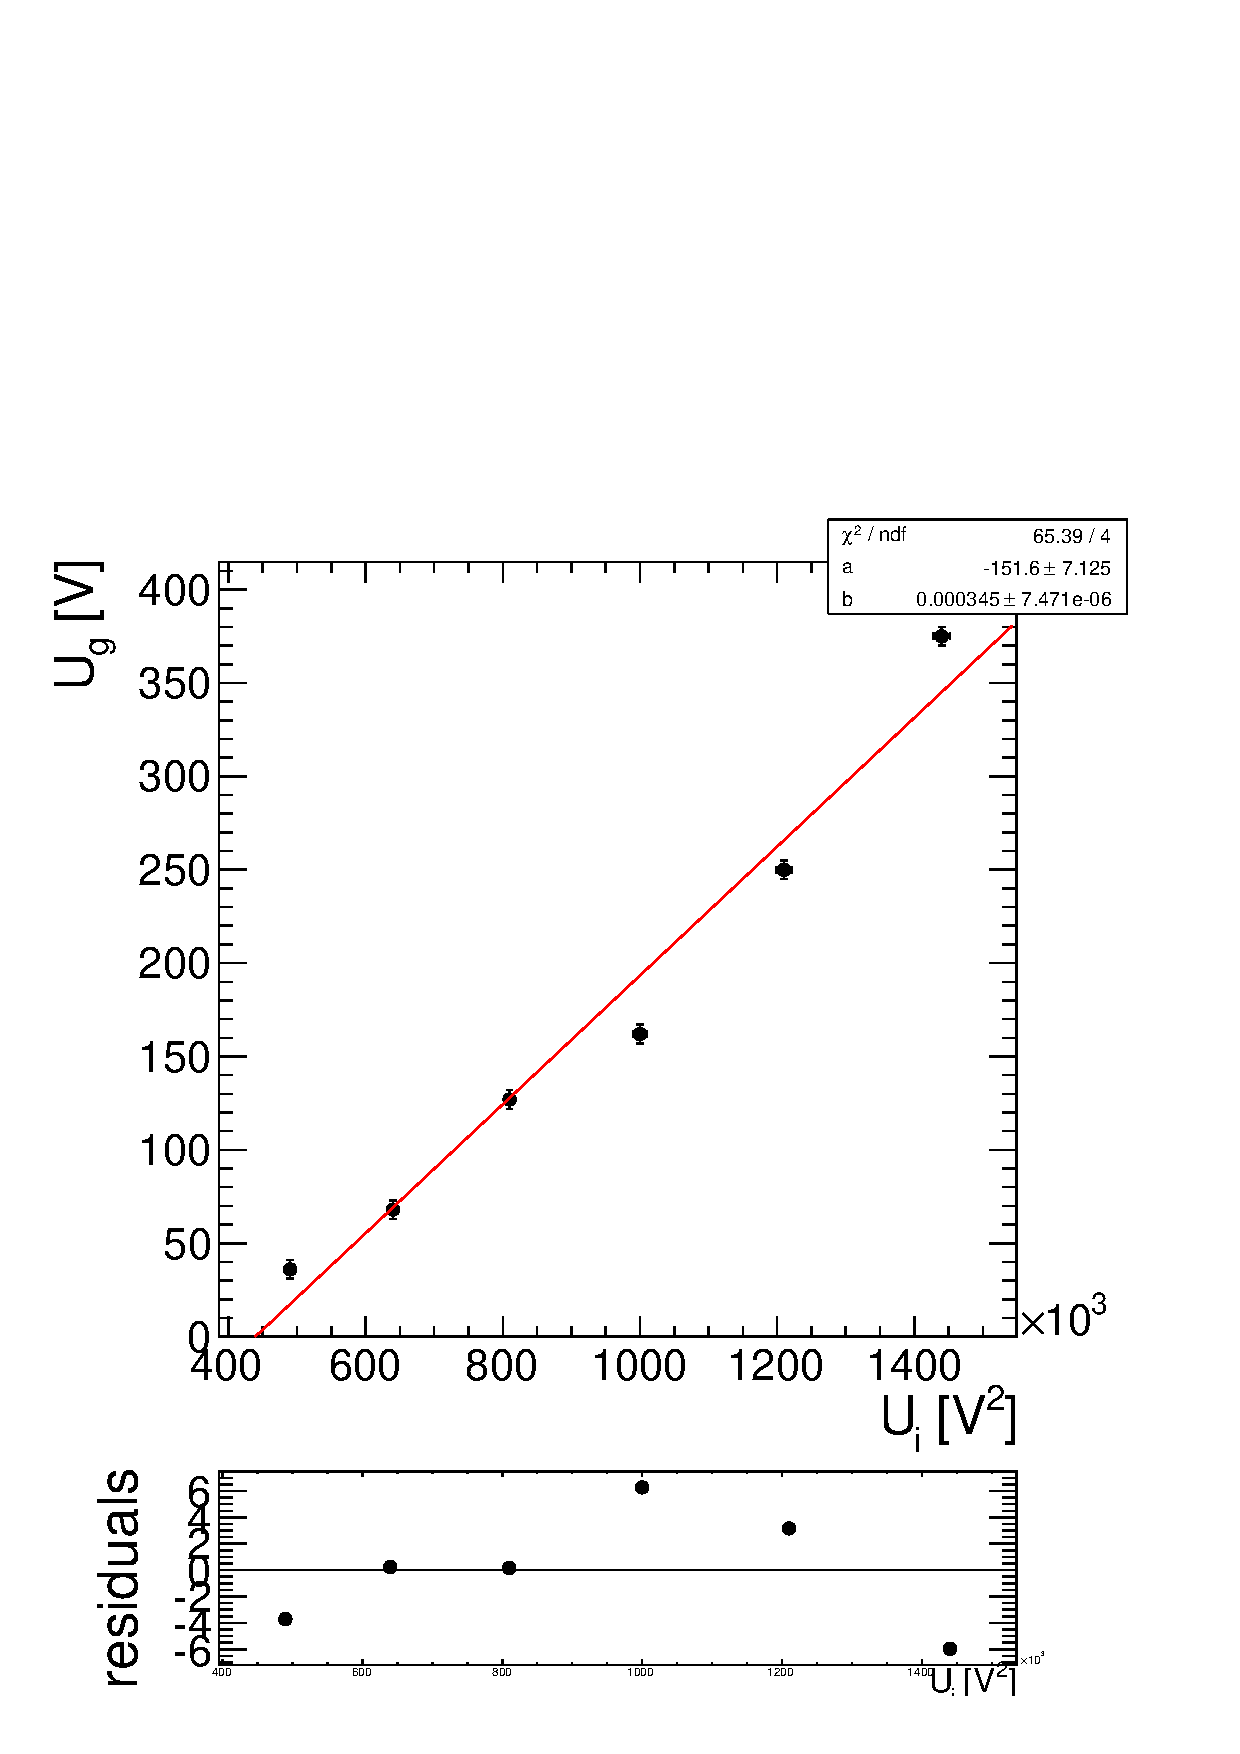
\includegraphics[height = 0.3\textheight]{../analyse/stabilitaet1.pdf}
		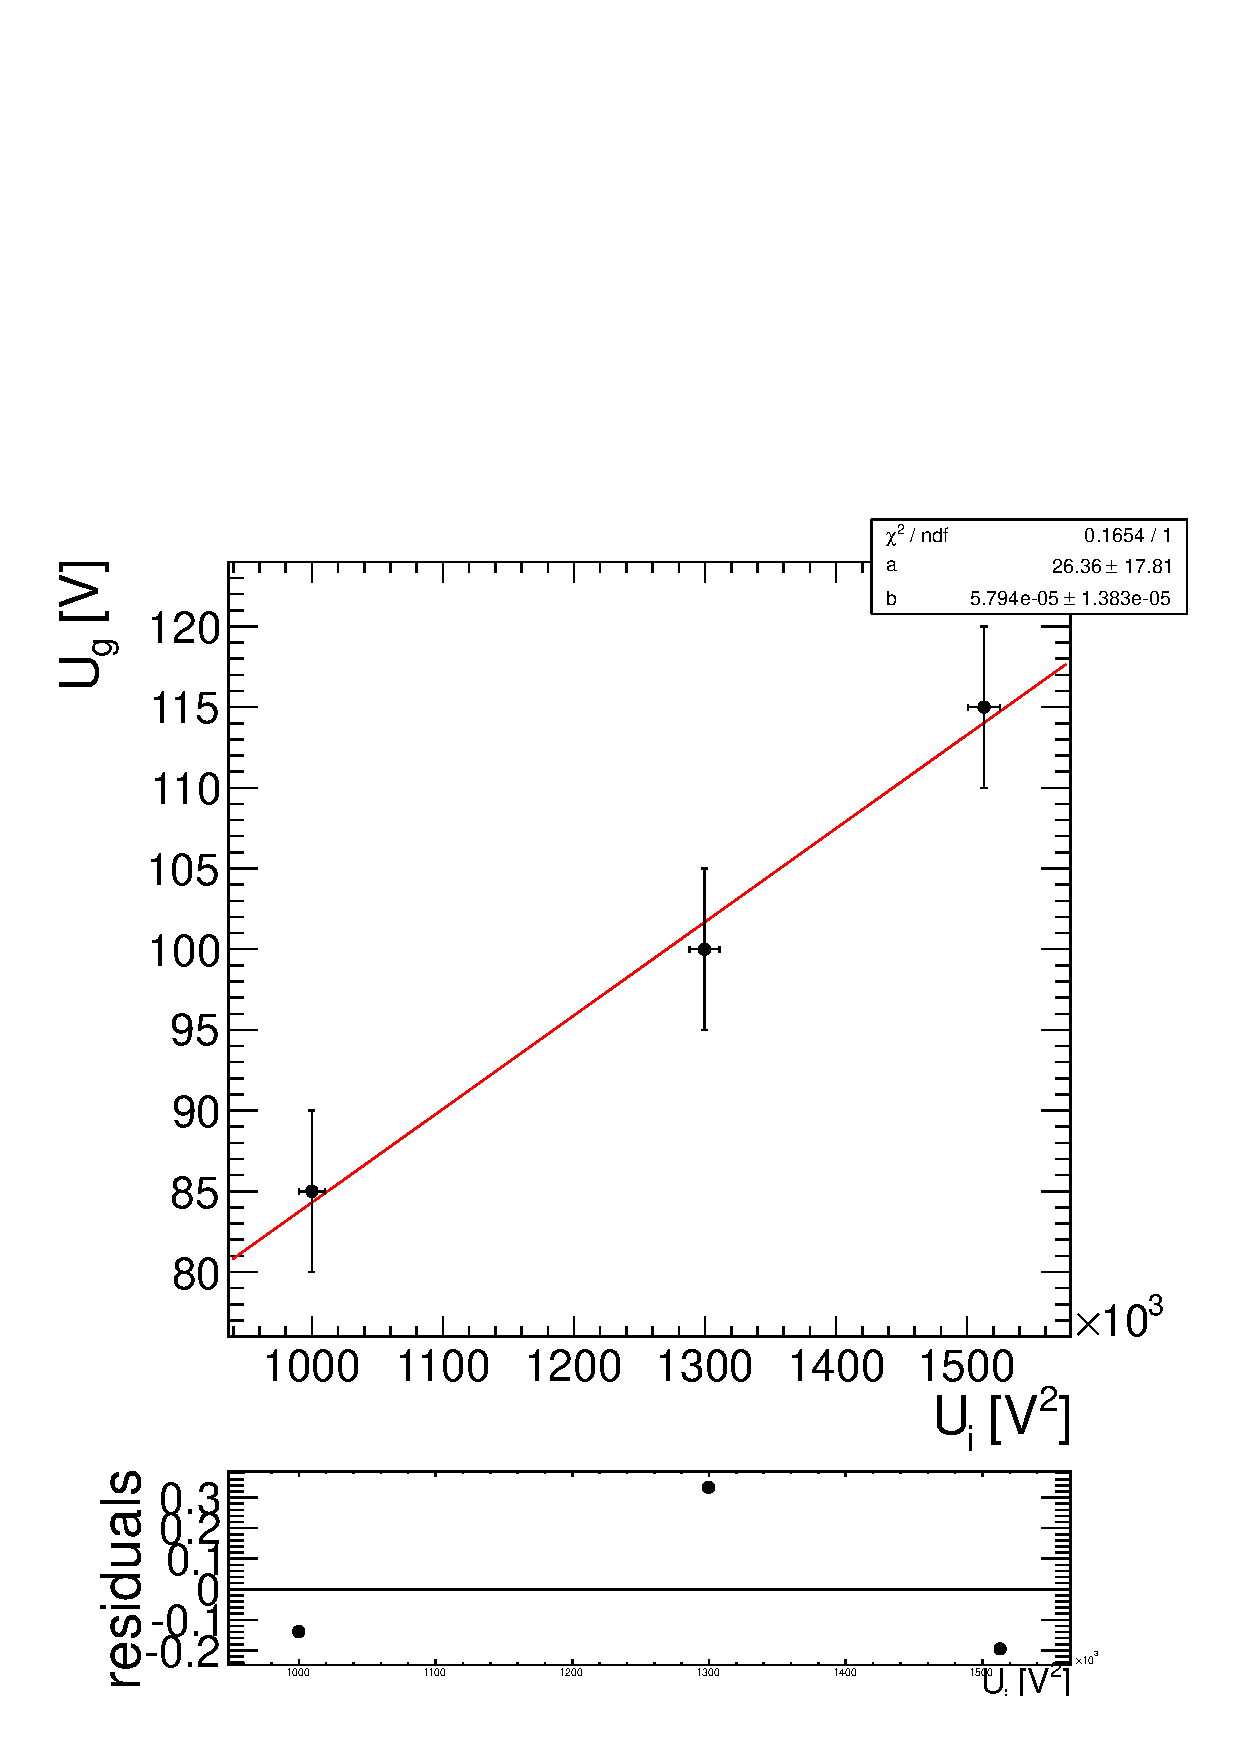
\includegraphics[height = 0.3\textheight]{../analyse/stabilitaet2.pdf}\\
		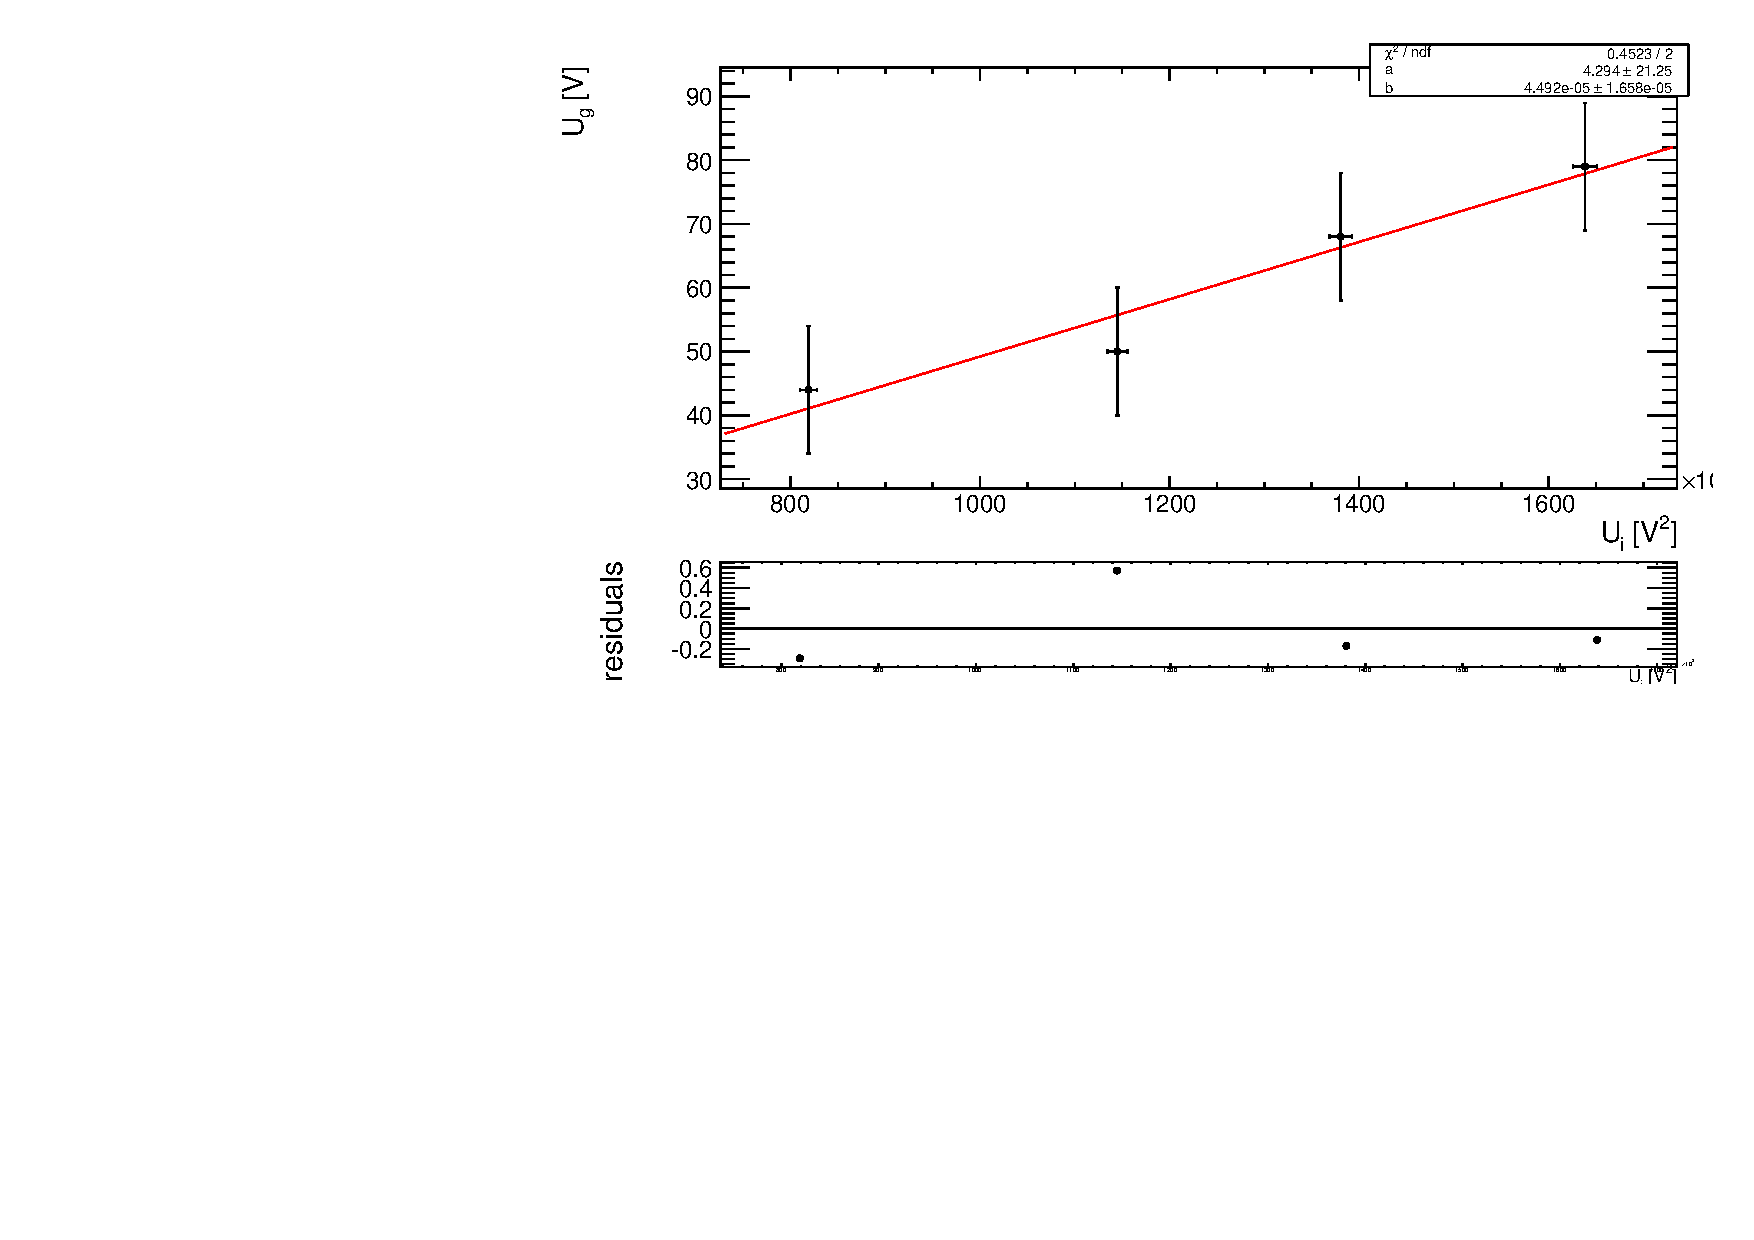
\includegraphics[height = 0.3\textheight]{../analyse/stabilitaet3.pdf}\\
		\caption{Lineare Regressionen zur Stabilitätsuntersuchung.
		Bei der oberen Messung ist der letzte Punkt nicht für den Fit verwendet worden, da bei dieser Spannug das Teilchen entkommen ist.
		Stattdessen kann man die Spannungsdifferenz zwischen eigentlichen Fluchtspannung und abgeschätzten Spannung ablesen.}
\end{figure}
Am $χ^2/ndf$ sieht man, dass die Spannungen tendenziell zu vorsichtig abgeschätzt wurden




\section{Vergleich der Messungen}

\section{Fazit}
Die Versuchsdurchführung war dadurch geprägt das die Spannungsquelle nur stark schwankende Ausgangsspannungen geliefert hat. Besonders ein reglemäßiges plötliches Abfallen der Fokussierspannung für ein 
Flächenpaar hat zu regelmäßigem Verlust der Teilchen geführt. Insbesondere die Resonanzmessung und die Stabiliätsmessung waren oft nicht durchzuführen, weil ein langfristiges einfangen der Teilchen nicht
möglich war.

% max 30 seiten
\end{document}
